%%%%%%%%%%%%%%%%%%%%%%%%%%%%%%%%%%%%%%%%%
% University/School Laboratory Report
% LaTeX Template
% Version 3.0 (4/2/13)
%
% This template has been downloaded from:
% http://www.LaTeXTemplates.com
%
% Original author:
% Linux and Unix Users Group at Virginia Tech Wiki 
% (https://vtluug.org/wiki/Example_LaTeX_chem_lab_report)
%
% License:
% CC BY-NC-SA 3.0 (http://creativecommons.org/licenses/by-nc-sa/3.0/)
%
%%%%%%%%%%%%%%%%%%%%%%%%%%%%%%%%%%%%%%%%%

%----------------------------------------------------------------------------------------
%	PACKAGES AND DOCUMENT CONFIGURATIONS
%----------------------------------------------------------------------------------------

\documentclass{article}

\usepackage[version=3]{mhchem} % Package for chemical equation typesetting
\usepackage{siunitx} % Provides the \SI{}{} command for typesetting SI units

\usepackage{graphicx}
\usepackage{caption}
\usepackage{subcaption}

\usepackage{float}

\usepackage[T1]{fontenc} % allow small bold caps

\setlength\parindent{0pt} % Removes all indentation from paragraphs

\renewcommand{\labelenumi}{\alph{enumi}.} % Make numbering in the enumerate environment by letter rather than number (e.g. section 6)

\usepackage[margin=1in]{geometry}

\usepackage{amssymb}

%\usepackage{times} % Uncomment to use the Times New Roman font

%----------------------------------------------------------------------------------------
%	Title
%----------------------------------------------------------------------------------------

\begin{document}
\pagenumbering{gobble}

\title{24.118: Paradox and Infinity}
\author{
  Ryan Lacey <rlacey@mit.edu>\\
  \footnotesize \texttt{Collaborator(s): Evan Thomas}
}
        
\maketitle
        


\begin{enumerate}
\item[1.]
	Define $P_n$ to be the $n^{th}$ prime. Eg. $P_0=2$, $P_1=3$, $P_2,=5$, etc\\
	
	For each $P_n$, if n is an even number, map it to n/2; and if n is an odd number, map it to -((n+1)/2).\\
	
	$P_0$ -> 0/2 = 0\\
	$P_1$ -> -(1+1)/2 = -1\\
	$P_2$ -> 2/2 = 1\\
	$P_3$ -> -(3+1)/2 = -2\\

\item[2.]
	We build a matrix of pairs $\langle n, m \rangle$  with $n$ specifying the row and $m$ specifying the column of the pair's cell. The setup is similar to the figure below, but with a natural number pair instead of a ratio of natural numbers. We can traverse the matrix in the same increasing diagonal manner as depicted in the diagram. This strategy ensures that we have a counting strategy (appropriate for the natural numbers) and that we are guaranteed to encounter all pairs of the nautral numbers.\\

\bigskip

\begin{figure}[!htb]
	\minipage{\textwidth}
		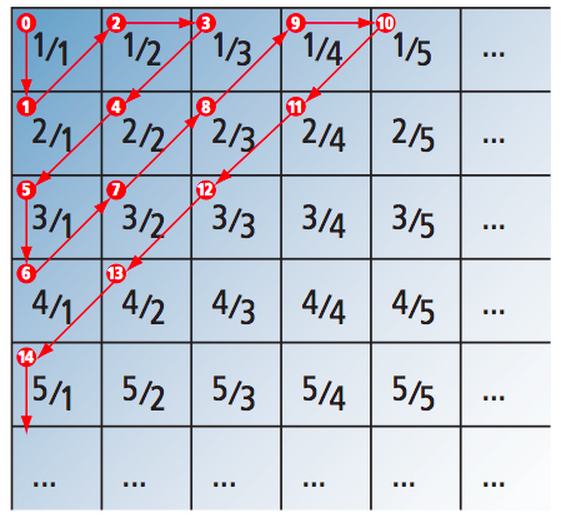
\includegraphics[width=\linewidth/3]{images/matrix.png}
		\caption{Matrix of rational numbers}
	\endminipage\hfill
\end{figure}

\newpage

\item[3.]
	Define a function from the interval [0,1) to the interval [0,$\infty$) as the following\\
	
	$f(x) = \dfrac{1}{1-x} - 1$\\
	
	Let's observe the extremes of the input range\\
	
	$f(0) = \dfrac{1}{1-0} - 1 = 0$\\
	
	$f(1) = \dfrac{1}{1-1} - 1 = \infty$\\
	
	$\therefore$ we can map anything from zero to infinity from the interval of zero to one.\\

\item[4.]
	skipped

\item[5.]
	Yes, there is a one-to-one correspondence between the natural numbers and nodes of the tree. We can traverse the tree by row and within each row visit the nodes. Each node visited will be assigned a natural number. Eg. Row 0 has one node, which is assigned value 0. Row 1 has two nodes, which are assigned values 1 and 2, etc.\\
	
	Proof for real numbers aplies to tree path, just under a different reprsentation. Proof taken from reals vs ration proof in the book.\\
	No, there is not a one-to-one correspondence between the paths of the trees and the natural numbers. Assume that it is possible to assign a different natural number to each path. If we have such an assignment, we can use it to make a list of all paths. We just let the first member of our list be the path that has been paired with the smallest natural number, the second member of our list be the path that has been paired with the second smallest natural number, and so forth. This allows us to build a table like the following\\

\begin{figure}[!htb]
	\minipage{\textwidth}
		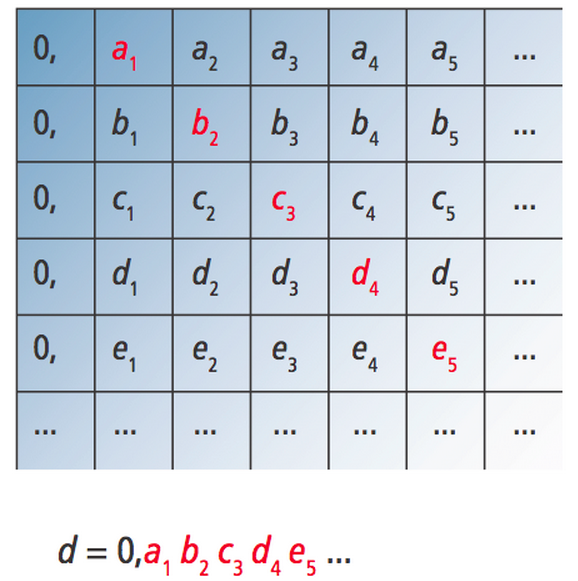
\includegraphics[width=\linewidth/3]{images/reals.png}
	\endminipage\hfill
\end{figure}

Now consider the number $d=0.a_1b_2c_3d_4e_5...$. We know that value $d$ must be different from the first member of our list because $f(a_1)$ is not equal to $a_1$, and it is different from the second member of our list because $f(b_2)$ is not equal to $b_2$, and so forth. But $d$ is a path of 0s and 1s. So we have succeeded in identifying a path not on our list. That contradicts our assumption. So our proof by reductio is complete.\\

\end{enumerate}

\end{document}